\documentclass{standalone}
\usepackage[paperwidth=\maxdimen,paperheight=\maxdimen]{geometry}
\usepackage{tikz}
\usepackage{graphicx}
\usetikzlibrary{shapes.geometric, arrows.meta, positioning}

\begin{document}


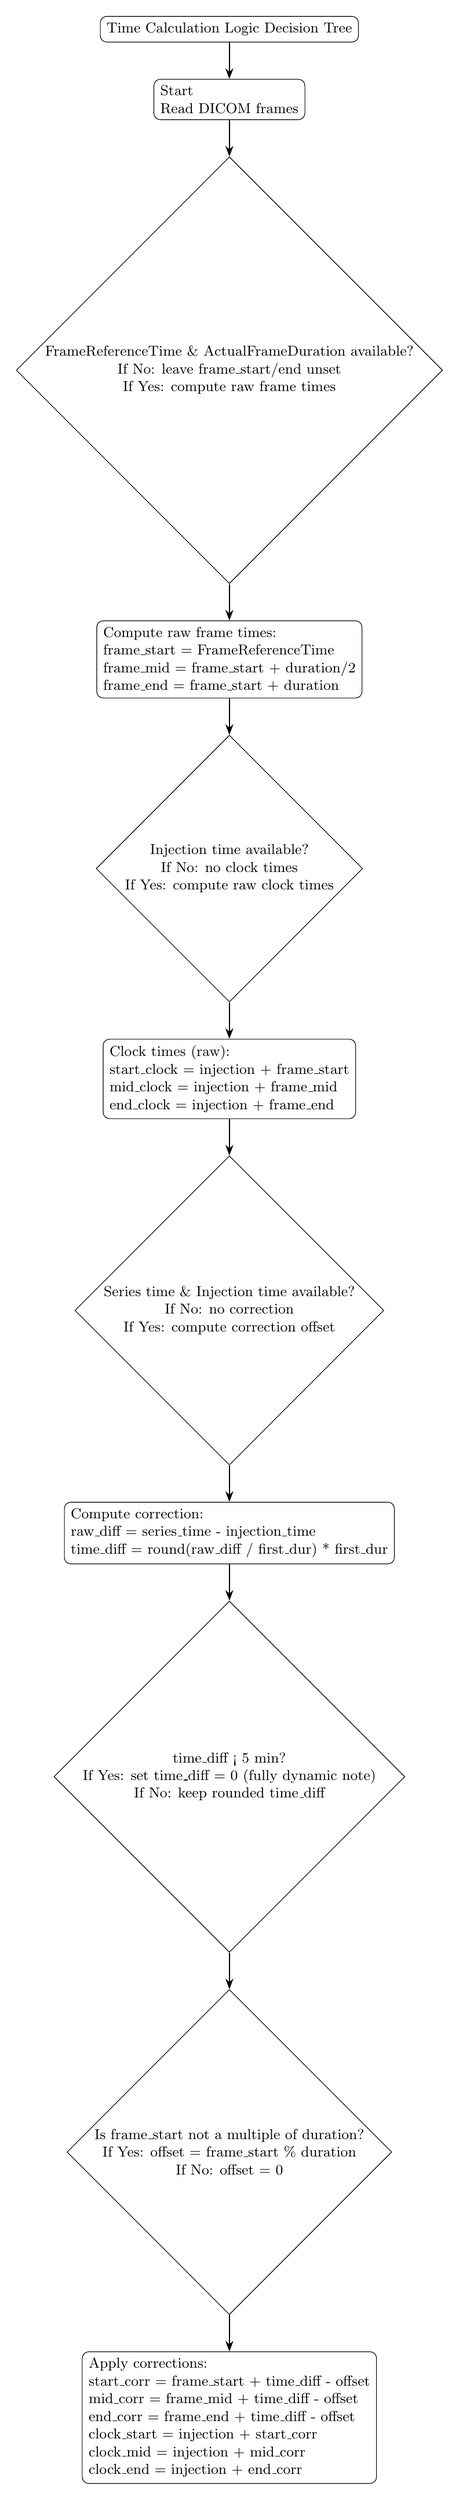
\begin{tikzpicture}[
  node distance=8mm,
  every node/.style={font=\small},
  decision/.style={diamond, draw, align=center, inner sep=1.5pt},
  process/.style={rectangle, draw, rounded corners, align=left, inner sep=4pt},
  arrow/.style={-{Stealth}, thick}
]

\node[process] (title) {Time Calculation Logic Decision Tree};

\node[process, below=of title] (start) {Start\\Read DICOM frames};

\node[decision, below=of start] (hasFrameRef)
{FrameReferenceTime \& ActualFrameDuration available?\\
If No: leave frame\_start/end unset\\
If Yes: compute raw frame times};

\node[process, below=of hasFrameRef] (calcRaw)
{Compute raw frame times:\\
frame\_start = FrameReferenceTime\\
frame\_mid = frame\_start + duration/2\\
frame\_end = frame\_start + duration};

\node[decision, below=of calcRaw] (hasInjectionTime)
{Injection time available?\\
If No: no clock times\\
If Yes: compute raw clock times};

\node[process, below=of hasInjectionTime] (clockRaw)
{Clock times (raw):\\
start\_clock = injection + frame\_start\\
mid\_clock = injection + frame\_mid\\
end\_clock = injection + frame\_end};

\node[decision, below=of clockRaw] (hasSeriesAndInjection)
{Series time \& Injection time available?\\
If No: no correction\\
If Yes: compute correction offset};

\node[process, below=of hasSeriesAndInjection] (prepCorrection)
{Compute correction:\\
raw\_diff = series\_time - injection\_time\\
time\_diff = round(raw\_diff / first\_dur) * first\_dur};

\node[decision, below=of prepCorrection] (smallDiff)
{time\_diff < 5 min?\\
If Yes: set time\_diff = 0 (fully dynamic note)\\
If No: keep rounded time\_diff};

\node[decision, below=of smallDiff] (applyOffset)
{Is frame\_start not a multiple of duration?\\
If Yes: offset = frame\_start \% duration\\
If No: offset = 0};

\node[process, below=of applyOffset] (applyCorrection)
{Apply corrections:\\
start\_corr = frame\_start + time\_diff - offset\\
mid\_corr = frame\_mid + time\_diff - offset\\
end\_corr = frame\_end + time\_diff - offset\\
clock\_start = injection + start\_corr\\
clock\_mid = injection + mid\_corr\\
clock\_end = injection + end\_corr};

% Arrows (straight down, centered)
\draw[arrow] (title) -- (start);
\draw[arrow] (start) -- (hasFrameRef);
\draw[arrow] (hasFrameRef) -- (calcRaw);
\draw[arrow] (calcRaw) -- (hasInjectionTime);
\draw[arrow] (hasInjectionTime) -- (clockRaw);
\draw[arrow] (clockRaw) -- (hasSeriesAndInjection);
\draw[arrow] (hasSeriesAndInjection) -- (prepCorrection);
\draw[arrow] (prepCorrection) -- (smallDiff);
\draw[arrow] (smallDiff) -- (applyOffset);
\draw[arrow] (applyOffset) -- (applyCorrection);

\end{tikzpicture}


\end{document}

\node[process, below right=of smallDiff, xshift=10mm] (keepRounded)
{Keep rounded time\_diff\\
Warn if rounded};

\node[decision, below=16mm of keepRounded] (applyOffset)
{Is frame\_start \\not multiple of duration?};

\node[process, below left=of applyOffset, xshift=-10mm] (offsetYes)
{offset = frame\_start \% duration};

\node[process, below right=of applyOffset, xshift=10mm] (offsetNo)
{offset = 0};

\node[process, below=16mm of offsetNo] (applyCorrection)
{Apply corrections to each frame:\\
start\_corr = frame\_start + time\_diff - offset\\
mid\_corr = frame\_mid + time\_diff - offset\\
end\_corr = frame\_end + time\_diff - offset\\
clock\_start = injection + start\_corr\\
clock\_mid = injection + mid\_corr\\
clock\_end = injection + end\_corr};

% Arrows
\draw[arrow] (start) -- (hasFrameRef);
\draw[arrow] (hasFrameRef) -- node[above left]{No} (noTiming);
\draw[arrow] (hasFrameRef) -- node[above right]{Yes} (calcRaw);

\draw[arrow] (calcRaw) -- (hasInjectionTime);
\draw[arrow] (hasInjectionTime) -- node[above left]{No} (noClock);
\draw[arrow] (hasInjectionTime) -- node[above right]{Yes} (clockRaw);

\draw[arrow] (clockRaw) -- (hasSeriesAndInjection);
\draw[arrow] (hasSeriesAndInjection) -- node[above left]{No} (noCorrection);
\draw[arrow] (hasSeriesAndInjection) -- node[above right]{Yes} (prepCorrection);

\draw[arrow] (prepCorrection) -- (smallDiff);
\draw[arrow] (smallDiff) -- node[above left]{Yes} (forceZero);
\draw[arrow] (smallDiff) -- node[above right]{No} (keepRounded);

\draw[arrow] (keepRounded) -- (applyOffset);
\draw[arrow] (forceZero) |- (applyOffset);

\draw[arrow] (applyOffset) -- node[above left]{Yes} (offsetYes);
\draw[arrow] (applyOffset) -- node[above right]{No} (offsetNo);

\draw[arrow] (offsetYes) |- (applyCorrection);
\draw[arrow] (offsetNo) -- (applyCorrection);

\end{tikzpicture}%
}



\end{document}